\documentclass{ximera}

\input{../preamble.tex}

\title{Symmetry}
\author{Jenny Sheldon}

\begin{document}

\begin{abstract}
We look at patterns within shapes.
\end{abstract}
\maketitle

\section{Activities for this section:} 
\link[Symmetry]{https://ximera.osu.edu/m4t/elementaryActivities/SemesterTwoPacket/elementaryActivities/ComparingShapes/Symmetry}

\section{Symmetry}

Broadly, symmetry is a way of recognizing, investigating, or designing patterns. It can also be a way of describing or even quantifying beauty, since \link[studies have shown]{https://www.psychologytoday.com/us/blog/beastly-behavior/201907/why-are-symmetrical-faces-so-attractive} that people with more symmetrical faces are generally considered more ``attractive''. Artists frequently play with symmetry in their art. And symmetry can show up all around us in both human-made objects as well as natural ones. For our purposes, however, symmetry gives us a chance to come back to rotations, reflections, translations, and congruence and see how these ideas apply to shapes individually. Symmetry will also give us another way to look at properties of shapes. You might take a few moments and review your notes on these concepts before we get started, or head back to the sections about \link[Transformations]{https://ximera.osu.edu/m4t/elementaryTeachersTwo/elementaryReading/ComparingShapes/Transformations} or \link[Congruence]{https://ximera.osu.edu/m4t/elementaryTeachersTwo/elementaryReading/ComparingShapes/Congruence}.

In general, a \dfn{symmetry} of a figure is a transformation that maps the figure onto itself. We'll explore some specific symmetries below. 

\section{Reflection symmetry}

A shape has a reflection symmetry over a particular line $L$ when we reflect the shape over the line $L$ and the result is congruent to the original without applying any translations. Said a bit more simply, we have a reflection symmetry with respect to line $L$ if, after reflection, we have the same shape in the same location. Thinking about what happens to the points when we reflect, each point in the original shape moves to a (possibly different) point in the original shape. In some sense, the points in the original shape are changing places with one another, but still forming the same shape. Let's look at a few examples.

\begin{example}
Let's consider a star shape and see if we can find some lines of reflection.
\begin{image}
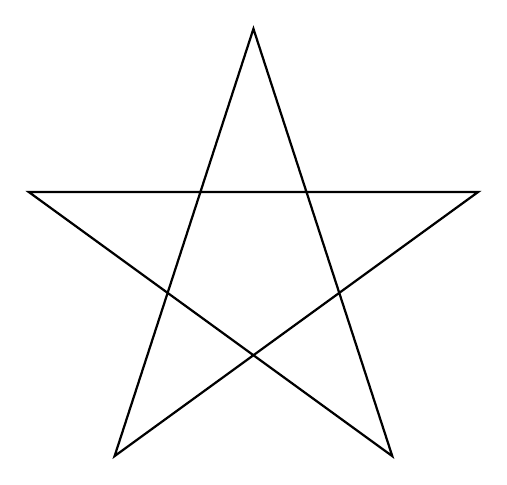
\begin{tikzpicture}
    % Coordinates for the points of the outer star
    \coordinate (A) at (90:3);
    \coordinate (B) at (162:3);
    \coordinate (C) at (234:3);
    \coordinate (D) at (306:3);
    \coordinate (E) at (18:3);
    
    % Draw the outline of the five-pointed star
    \draw[thick] (A) -- (C) -- (E) -- (B) -- (D) -- cycle;
    

\end{tikzpicture}
\end{image}
When we reflect, we can think about this like taking our original shape and \wordChoice{\choice[correct]{folding} \choice{turning} \choice{shifting}} it along the line of reflection. If that line of reflection is a line of symmetry, the two halves of the shape will exactly match up when we do. Remember that this is telling us about both sides of the fold, not just one! We need to think about what's happening to the entire plane, not just half of it. Let's take a look at the next image.

\begin{image}
\begin{tikzpicture}
    % Coordinates for the points of the star
    \coordinate (A) at (90:3);
    \coordinate (B) at (162:3);
    \coordinate (C) at (234:3);
    \coordinate (D) at (306:3);
    \coordinate (E) at (18:3);

    % Draw the outline of the five-pointed star
    \draw[thick] (A) -- (C) -- (E) -- (B) -- (D) -- cycle;
    
    % Draw the lines of reflection
    \draw[dashed] (A) -- ($ (C)!.5!(D) $) node[below]{$L_1$}; % Vertical line
    \draw[dashed] (C) -- ($ (A)!.5!(E) $) node[above right]{$L_3$}; % Line from bottom left to top right
    \draw[dashed] (E) -- ($ (B)!.5!(C) $) node[below]{$L_5$}; % Line from bottom right to top left
    \draw[dashed] (B) -- ($ (D)!.5!(E) $) node[below]{$L_2$}; % Line from top left to bottom right
    \draw[dashed] (D) -- ($ (A)!.5!(B) $) node[above left]{$L_4$}; % Line from top right to bottom left
\end{tikzpicture}
\end{image}
We have drawn dashed lines through each of the points of the star and labeled the lines $L_1$ through $L_5$. If we fold the star along any of these lines, the two halves will match up exactly. So, each of these lines is a line of symmetry for the star once we unfold again. We have a total of $\answer[given]{5}$ lines of symmetry in this case.

\end{example}

Next, let's investigate a question where we have some examples of lines of symmetry and some examples of reflection lines that are not lines of symmetry.

\begin{question}
Which of the following are lines of reflection symmetry for the square $ABCD$? Select all that apply.
\begin{image}
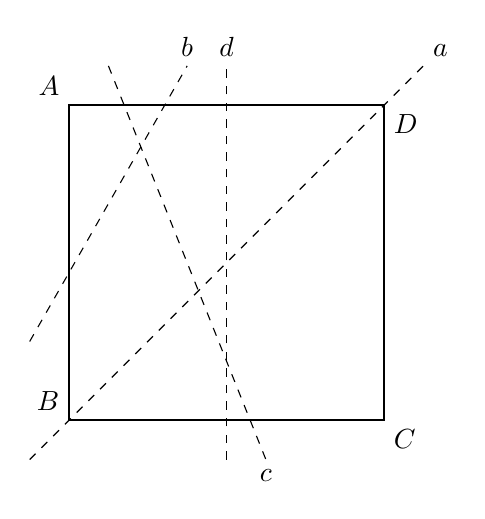
\begin{tikzpicture}
\draw[thick] (0,0)--(4,0)--(4,4)--(0,4)--(0,0);
\draw[dashed] (-0.5, -0.5)--(4.5, 4.5) node[above right]{$a$};
\draw[dashed] (-0.5, 1)--(1.5, 4.5) node[above]{$b$};
\draw[dashed] (0.5, 4.5)--(2.5, -0.5) node[below]{$c$};
\draw[dashed] (2, -0.5)--(2, 4.5) node[above]{$d$};
\node[above left] at (0,4) {$A$};
\node[above left] at (0,0) {$B$};
\node[below right] at (4,0) {$C$};
\node[below right] at (4,4) {$D$};
\end{tikzpicture}
\end{image}
\end{question}

\begin{selectAll}
\choice[correct]{Line $a$ through points $B$ and $D$}
\choice{Line $b$ through side $AB$ and side $AD$}
\choice{Line $c$ through side $AD$ and side $BD$ but not the midpoints}
\choice[correct]{Line $d$ through the midpoints of sides $AD$ and $BD$}
\end{selectAll}


\section{Rotation symmetry}


A shape has rotation symmetry when we can choose a point $O$ for the center of rotation and an angle $a$ of rotation where the result of rotating the shape by angle $a$ about point $O$ is a shape congruent to the original without applying any translations. Again, said more simply, we have the same shape in the same location, or the points are changing places within the same shape. It's time for more examples!

\begin{example}
Let's start with a figure that's a bit like an equilateral triangle, but it has other little triangles stuck on the sides near each vertex.
\begin{image}
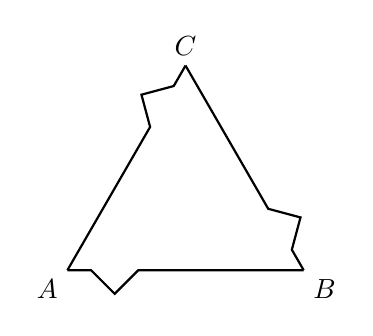
\begin{tikzpicture}
	\coordinate (C) at (1.5,{3*sqrt(3)/2});
    \draw[thick] (0,0)--(0.3,0)--(0.6,-0.3)--(0.9,0)--(3,0);


    % Rotate the shape two more times to achieve order 3 rotational symmetry
    \begin{scope}[shift={(3,0)}, rotate=120]
         \draw[thick] (0,0)--(0.3,0)--(0.6,-0.3)--(0.9,0)--(3,0);
    \end{scope}
    \begin{scope}[shift={(C)}, rotate=240]
         \draw[thick] (0,0)--(0.3,0)--(0.6,-0.3)--(0.9,0)--(3,0);
    \end{scope}
    \node[below left] at (0,0) {$A$};
    \node[below right] at (3,0) {$B$};
    \node[above] at (C) {$C$};
\end{tikzpicture}
\end{image}

When we rotate, we are thinking about \wordChoice{\choice{folding} \choice[correct]{turning} \choice{shifting}} 
around a chosen point. We need to find a point around which to rotate, and since we want to end up with the same 
shape in the same spot, we want  to use 
\wordChoice{\choice{vertex $A$} \choice{vertex $B$} \choice{vertex $C$} \choice[correct]{the middle of the figure}}. 
We have some choices for the angle in this case, since when the shape ends up in the same spot we need vertices to 
match up with vertices after rotating. So, if we rotate vertex $A$ to match up with vertex $B$ we would rotate $120\degree$ counterclockwise:

\begin{image}
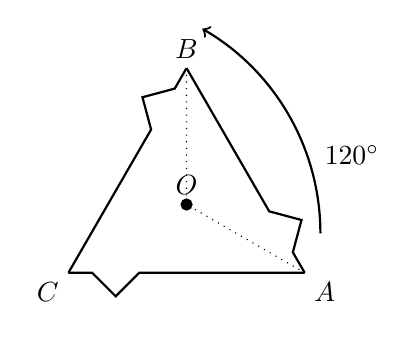
\begin{tikzpicture}
	\coordinate (C) at (1.5,{3*sqrt(3)/2});
	\coordinate (center) at (1.5,{sqrt(3)/2});
    \draw[thick] (0,0)--(0.3,0)--(0.6,-0.3)--(0.9,0)--(3,0);


    % Rotate the shape two more times to achieve order 3 rotational symmetry
    \begin{scope}[shift={(3,0)}, rotate=120]
         \draw[thick] (0,0)--(0.3,0)--(0.6,-0.3)--(0.9,0)--(3,0);
    \end{scope}
    \begin{scope}[shift={(C)}, rotate=240]
         \draw[thick] (0,0)--(0.3,0)--(0.6,-0.3)--(0.9,0)--(3,0);
    \end{scope}

    \node[below left] at (0,0) {$C$};
    \node[below right] at (3,0) {$A$};
    \node[above] at (C) {$B$};
    
    \filldraw (center) circle (2pt) node[above] {$O$};
% Draw the arc for rotation
    \draw[thick, ->] (3.2, 0.5) arc[start angle=0, end angle=60, radius=3];
    \node at (3.6, 1.5) {$120^{\circ}$};
    \draw[dotted] (C)--(center)--(3,0);
\end{tikzpicture}
\end{image}
We have shown the rotation angle's vertex and two rays with dotted lines in the figure. Notice that the vertices $A$, $B$, and $C$ have changed places, but the entire figure looks the same as when we started.

We can rotate again using the central point $O$ another $120\degree$ (for a total of $240\degree$ from the start).
\begin{image}
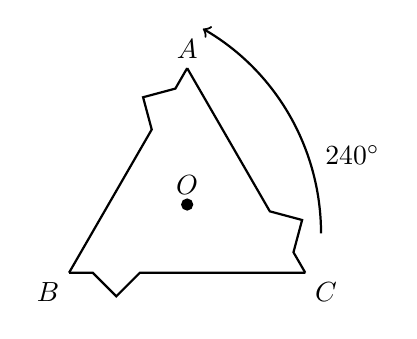
\begin{tikzpicture}
	\coordinate (C) at (1.5,{3*sqrt(3)/2});
	\coordinate (center) at (1.5,{sqrt(3)/2});
    \draw[thick] (0,0)--(0.3,0)--(0.6,-0.3)--(0.9,0)--(3,0);


    % Rotate the shape two more times to achieve order 3 rotational symmetry
    \begin{scope}[shift={(3,0)}, rotate=120]
         \draw[thick] (0,0)--(0.3,0)--(0.6,-0.3)--(0.9,0)--(3,0);
    \end{scope}
    \begin{scope}[shift={(C)}, rotate=240]
         \draw[thick] (0,0)--(0.3,0)--(0.6,-0.3)--(0.9,0)--(3,0);
    \end{scope}

    \node[below left] at (0,0) {$B$};
    \node[below right] at (3,0) {$C$};
    \node[above] at (C) {$A$};
    
    \filldraw (center) circle (2pt) node[above] {$O$};
% Draw the arc for rotation
    \draw[thick, ->] (3.2, 0.5) arc[start angle=0, end angle=60, radius=3];
    \node at (3.6, 1.5) {$240^{\circ}$};
\end{tikzpicture}
\end{image}
Again, the vertices have changed places, but the overall shape remains the same. If we rotated one more $120\degree$ around $O$, that 
would be $360\degree$ from the start, and the shape would turn all the way around and return to the start. We won't draw this one, 
but you should visualize it. Overall, for this shape, we can rotate it by $120\degree$ around $O$ a total of $\answer[given]{3}$ times to return to the start. Notice that $3 \times 120 = 360$, so after the three rotations we have made a full turn which should return us to the start.

\end{example}



There are a few things to notice about this example. First, if we consider any shape at all, we can always rotate about its center 
by $360\degree$ and return the shape to its original state. We don't particularly consider this a rotation symmetry since it's not 
very interesting mathematically. However, this is related to the second observation we want to make. When we rotate, we can keep track 
of how many times the figure matches up with its original state, including the final time when we hit $360\degree$. In the previous 
example, we could rotate by $120\degree$ three times including that final time when came back to the original. This number of times 
the shape matches up with the original state is called the \dfn{order} of the rotation.
\begin{question}
What is the order of the rotation symmetry in the previous example? 

\begin{prompt}
The rotation symmetry has order $\answer[given]{3}$.
\end{prompt}
 \end{question}

Shapes can sometimes have more than one type of symmetry.
\begin{question}
True or false: the example above of the triangle with extra pieces also has reflection symmetry.
\begin{multipleChoice}
\choice{True}
\choice[correct]{False}
\end{multipleChoice}

True or false: all of the examples in the reflection section also have rotational symmetry.
\begin{multipleChoice}
\choice[correct]{True}
\choice{False}
\end{multipleChoice}
\end{question}

\begin{question}
What is the order of the rotation symmetry for the star example in the ``Reflection symmetry'' section?
\begin{prompt}
$\answer[given]{5}$
\end{prompt}

What is the order of the rotation symmetry of a regular octagon? (Please draw one to help you with this question!)
\begin{prompt}
$\answer[given]{8}$
\end{prompt}

\end{question}


\begin{question}
Pause and think: how could you draw a shape that has reflection symmetry but does not have rotation symmetry?
\begin{freeResponse}
Draw some pictures in your notes, and remind yourself here where you drew them.
\end{freeResponse}
\end{question}


\section{Translation symmetry}

A shape has a translation symmetry with respect to a particular distance and direction $V$ when we translate the shape using $V$ and the result is congruent to the original without applying any translations. Remember that we usually express $V$ as a vector with both length and direction. As with reflections and rotations, we are looking for the same shape in the same location. Examples are a little more complicated in this case, but I think we can make this work.

\begin{example}
Here is a design that has translation symmetry.
\begin{image}
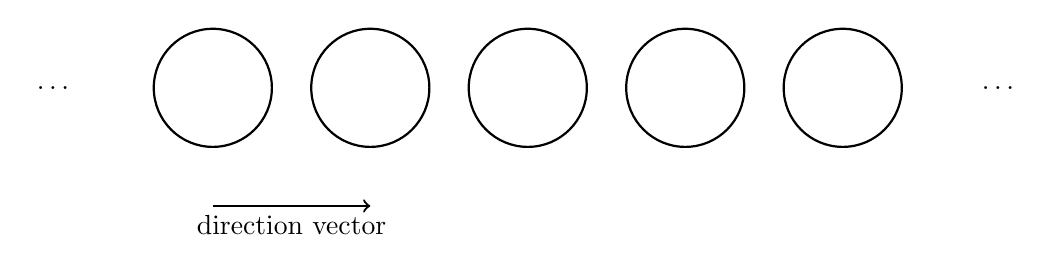
\begin{tikzpicture}
\foreach \x in {0, 2, 4, 6, 8} \draw[thick] (\x,0) circle (0.75cm);
\node at (-2, 0) {\dots};
\node at (10, 0) {\dots};
\draw[thick, ->] (0, -1.5) -- (2, -1.5);
\node[below] at (1, -1.5) {direction vector};
\end{tikzpicture}
\end{image}
In the figure, we see a sequence of circles. The dots at either end indicate that the pattern keeps going forever in each direction. So, this is a line of circles that is infinitely long. We also see a direction vector which tells us to translate directly east, and the vector moves the center of one circle to the next.

A translation can be thought of as a  \wordChoice{\choice{fold} \choice{turn} \choice[correct]{shift}}, and the vector tells us how to do this. Since this particular vector moves the center of one circle to the center of the next circle, after translating the design will look \wordChoice{\choice[correct]{exactly the same as } \choice{different from}} the original design.

\end{example}
With translation symmetry, we need the design to look exactly the same as the original. Since translations typically shift the design from one place to the next (not leaving the shape in the same location), we typically have to have a design that doesn't have ends in order to have translation symmetry. Our example above doesn't have ends because it goes on forever to the left and the right.

\begin{question}
The example with the star (in the reflection section) has translation symmetry.
\begin{multipleChoice}
\choice{True}
\choice[correct]{False}
\end{multipleChoice}

If we took the star example and made  an infinite line of stars, we could form a design with translation symmetry.
\begin{multipleChoice}
\choice[correct]{True}
\choice{False}
\end{multipleChoice}
\end{question}


\section{Symmetry and properties}

We can use what we've now learned about symmetry to think about properties of quadrilaterals. The most important idea we need here is to remember that a symmetry is built from reflections, rotations and translations, and we know that these particular transformations don't change lengths and they don't change angles.

\begin{example}
Let's show that the diagonals of a square are congruent to one another. 

We'll draw a square $ABCD$ whose center point is $O$ along with its diagonals $AC$ and $BD$.
\begin{image}
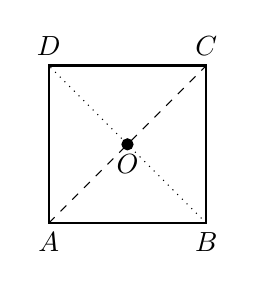
\begin{tikzpicture}
	\draw[fill=black] (0,0) circle (2pt) node[below] {$O$};
	\draw[thick] (-1, -1) rectangle (1,1);
	\node[below] at (-1,-1) {$A$};
	\node[below] at (1, -1) {$B$};
	\node[above] at (1,1) {$C$};
	\node[above] at (-1,1) {$D$};
	\draw[dashed] (-1,-1)--(1,1);
	\draw[dotted] (1,-1)--(-1,1);
\end{tikzpicture}
\end{image}

Next, we will use a rotational symmetry.  We \wordChoice{\choice{reflect} \choice[correct]{rotate} \choice{translate}} the square $90^{\circ}$ counterclockwise about point $\answer[given]{O}$, we get back the same square that we started with. It's the same shape, in the same location. However, after we rotated, the locations of the points have moved. Point $A$ moves to the original location of point $\answer[given]{B}$, point $B$ moves to the original location of point $\answer[given]{C}$, point $C$ moves to the original location of point $\answer[given]{D}$, and point $D$ moves to the original location of point $A$.

\begin{image}
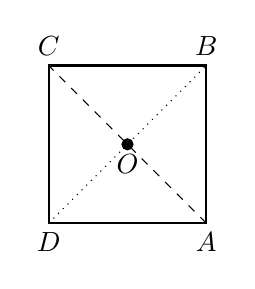
\begin{tikzpicture}
	\draw[fill=black] (0,0) circle (2pt) node[below] {$O$};
	\draw[thick] (-1, -1) rectangle (1,1);
	\node[below] at (-1,-1) {$D$};
	\node[below] at (1, -1) {$A$};
	\node[above] at (1,1) {$B$};
	\node[above] at (-1,1) {$C$};
	\draw[dotted] (-1,-1)--(1,1);
	\draw[dashed] (1,-1)--(-1,1);
\end{tikzpicture}
\end{image}

What does this mean for our diagonals? They have exchanged places in the square. However, since we know we have the same square, these lengths must exactly match up with one another, so they are congruent.

\end{example}

Remember that we could prove the same fact with our triangle congruence criteria. Symmetry gives us another way of thinking about the same fact.



\section{Other examples of symmetry}

Symmetry is prevalent in many other examples. There are two we'd like to quickly mention to wrap up this section and we encourage you to explore these examples as well as others you find in your everyday life. 

First, symmetry shows up in many ways in dance. In fact, dance is sometimes used to teach symmetry in the classroom. You can check out an \link[example lesson]{https://artsnowlearning.org/project/using-movement-and-dance-to-explore-symmetry-2-4/} or a \link[video of children exploring dance and symmetry]{https://www.youtube.com/watch?v=mF1CyYvMdgM}. Both of these examples focus on reflection symmetry. Can you think of ways that the ideas of rotational or translational symmetry could also be involved?

Second, symmetry shows up in objects called \dfn{fractals}. A fractal is a shape that's similar to itself but at a different scale. In other words, we are thinking about dilation symmetry. Fractals have applications in mathematics, like trying to \link[model chaos]{https://fractalfoundation.org/resources/what-are-fractals/} or to \link[model nature (video)]{https://www.youtube.com/watch?v=rGwwydEWLiI&t=48s}. Fractals are also found in \link[art]{https://en.wikipedia.org/wiki/Fractal_art}, in both traditional and digital media. And zooming in on them can make some really \link[interesting videos]{https://www.youtube.com/watch?v=9M7dTmvJxwA}!



\end{document}
